\documentclass[a4paper,12pt,twocolumn]{article}

\usepackage{times}
\usepackage[utf8]{inputenc}
\usepackage[brazil]{babel}
\usepackage[a4paper,margin=2cm,columnsep=1cm]{geometry}
\usepackage{authblk}
\usepackage{titlesec}
\usepackage[pdftex]{graphicx}
\usepackage{mathtools}
\usepackage{amsmath}
\usepackage{enumitem}
\usepackage[font={small}]{caption}

\topmargin      0.0cm
\headheight     0.0cm
\headsep        0.0cm
\oddsidemargin  0.0cm
\evensidemargin 0.0cm
\textheight     22.86cm
\textwidth      16.51cm

\graphicspath{{images/}}
\titleformat*{\section}{\normalsize\bfseries\filcenter}
\titleformat*{\subsection}{\normalsize\bfseries\filcenter}

\renewcommand{\figurename}{\small Figure}
\newcommand{\figureref}[1]{Fig. (\ref{fig:#1})}
\newcommand{\equationref}[1]{Eq. (\ref{eq:#1})}
\newcommand{\bigsum}{\displaystyle\sum}


\begin{document}

\title{\textbf{Resumo de Aprendizagem de Máquina 2014-2}}
\author{
    \textbf{Eduardo M. B. de A. Tenório}\\
    \small{\texttt{embat@cin.ufpe.br}}
}
\affil{\large CIn-UFPE}
\date{}

\maketitle


\begin{abstract}
\begin{itshape}
Este documento tem por finalidade ser um resumo dos assuntos abordados na disciplina \emph{Aprendizagem de Máquina} do período 2014-2 do CIn-UFPE, ministrada pelos professores Francisco Carvalho e Teresa Ludermir. A maioria do documento referencia o livro ``Pattern Classification", de Duda, Hart e Stork. Os códigos utilizados como exercício de fixação encontram-se em \normalfont{https://github.com/embatbr/aprendizagem}.
\end{itshape}
\end{abstract}


\section{Teoria da Decisão Bayesiana}

Teoria da Decisão Bayesiana é uma abordagem estatística para a classificação de
padrões, baseada em quantificar os tradeoffs associados a tomar uma determinada
decisão (classificar) utilizando probabilidade e considerando os custos associados.

O \textbf{estado natural} é denotado por $\omega$, de modo que $\omega = \omega_i$, para $i = 1, 2, ..., c$, significa que o exemplo foi classificado como pertencente à classe $\omega_i$. Cada uma dessas classes possui uma \textbf{probabilidade a priori} $P(\omega_i)$, com

\begin{equation}
    \sum_{i=1}^{c} P(\omega_i) = 1,
    \label{eq:sum_priori_prob_to_one}
\end{equation}

\noindent refletindo o conhecimento prévio da chance de um elemento da classe $\omega_i$ aparecer. A \textbf{regra de decisão} seria: Decida $\omega_i$ para $\max_i P(\omega_i)$. Neste caso a classe $\omega_i$ sempre é escolhida e a probabilidade de erro é dada por:

\begin{equation}
    P_{err}(\omega_i) = 1 - P(\omega_i).
    \label{eq:prob_i_error}
\end{equation}

Utilizando uma característica $x$ que seja contínua e aleatória, sua \textbf{densidade de probabilidade estado-condicional} é dada por $p(x|\omega)$. Logo, a diferença entre $p(x|\omega_i)$ e $p(x|\omega_j)$ descreve a diferença da característica $x$ entre as populações das classes $\omega_i$ e $\omega_j$.

\begin{figure}[ht]
    \centering
    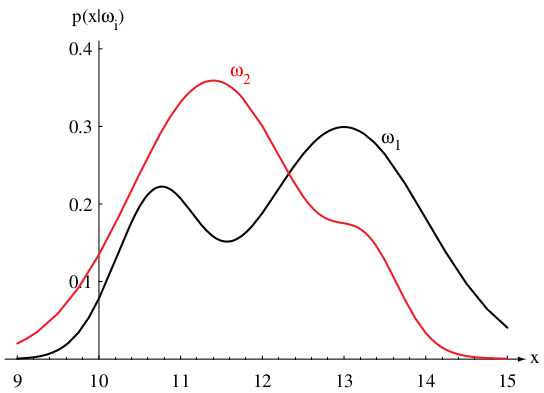
\includegraphics[scale=0.4]{state-conditional_pdf}
    \caption{Para $\omega_i = \omega_2$, é mais frequente observar $x$ entre 11 e 12 que $x = 13$ (valor mais provável se $\omega_i = \omega_1$).}
    \label{fig:state-conditional_pdf}
\end{figure}

Sabendo $P(\omega_i)$ e $p(x|\omega_i)$, e medindo um valor $x$, a probabilidade conjunta de achar um padrão na classe $\omega_i$ e com $x$ é dado por: $p(\omega_i,x) = P(\omega_i|x)p(x) = p(x|\omega_i)P(\omega_i)$, que pela \textbf{fórmula de Bayes} fica:

\begin{equation}
    P(\omega_i|x) = \frac{p(x|\omega_i)P(\omega_i)}{p(x)},
    \label{eq:bayes}
\end{equation}

\noindent com a evidência para $c$ classes

\begin{equation}
    p(x) = \sum_{j=1}^c p(x|\omega_j)P(\omega_j).
    \label{eq:bayes}
\end{equation}

A fórmula de Bayes pode ser expressa em português como

\begin{equation}
    posteriori = \frac{verossimilhanca \times priori}{evidencia}.
    \label{eq:bayes}
\end{equation}

\figureref{posteriori_prob} mostra a probabilidade a posteriori das classes $\omega_1$ e $\omega_2$ para um conjunto de valores de $x$. A regra de decisão muda para: Decida $\omega_i$ se $\omega_i$ minimiza $P(erro|x)$, onde

\begin{equation}
    P(erro|x) = \sum_{j\neq i} P(\omega_j|x),
    \label{eq:bayes}
\end{equation}

\noindent ou simplesmente $P(erro|x) = 1 - P(\omega_i|x)$. Então a regra torna-se: Decida $\omega_i$ para $\max_i P(\omega_i|x)$

\begin{figure}[ht]
    \centering
    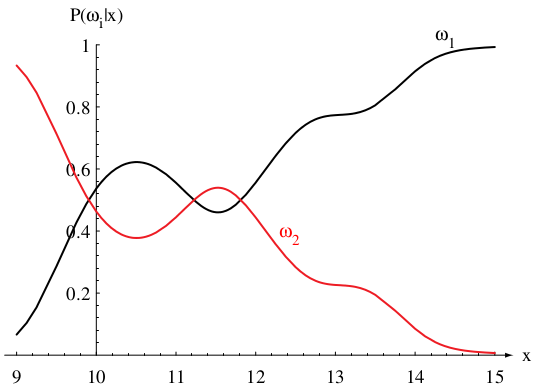
\includegraphics[scale=0.4]{posteriori_prob}
    \caption{Probabilidades a posteriori para $P(\omega_1) = \frac{2}{3}$ e $P(\omega_2) = \frac{1}{3}$, e para as densidades de probabilidade estado-condicional mostradas em \figureref{state-conditional_pdf}.}
    \label{fig:posteriori_prob}
\end{figure}

Esta regra minimiza a probabilidade média de erro, dada por

\begin{equation}
    P(erro) = \int_{-\infty}^{\infty} P(erro|x)p(x) dx.
    \label{eq:bayes}
\end{equation}

\end{document}